\chapter{مفاهیم پایه}

\section{معماری \lr{NFV}}
با توجه به استاندارد \lr{ETSI} معماری \lr{NFV}
از سه عنصر کلیدی تشکیل شده است.
زیرساخت مجازی‌سازی کارکردهای شبکه،
کارکردهای مجازی شبکه‌ای و
\lr{NFV MANO}.
این اجزا در شکل \cref{fig.1} نمایش داده شده‌اند.

\begin{figure}[!h]
\center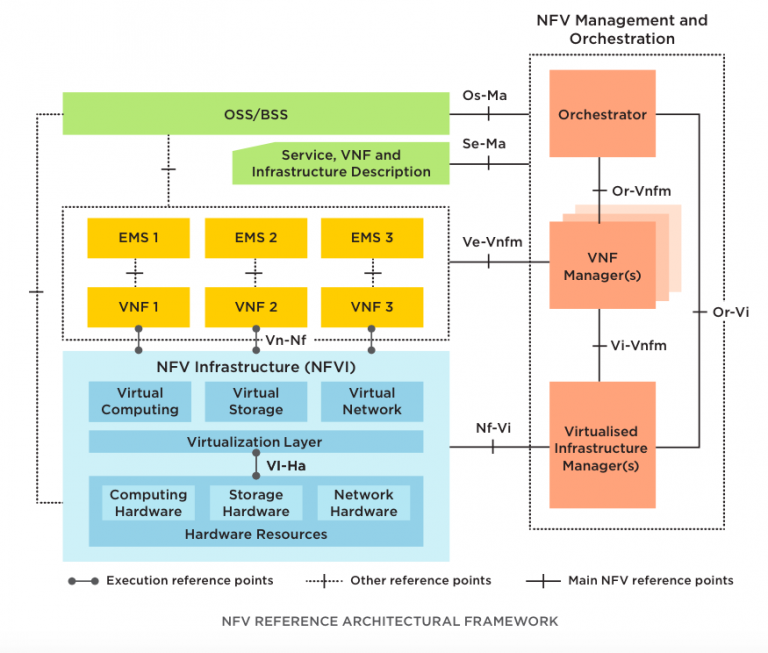
\includegraphics[scale=.5]{images/nfv-arch}
\caption{معماری مجازی‌سازی کارکردهای شبکه
}\label{fig.1}
\end{figure}

\section{زیرساخت مجازی‌سازی کارکردهای شبکه}
زیرساخت مجازی‌سازی کارکردهای شبکه ترکیبی از منابع نرم‌افزاری و سخت‌افزاری است
که محیطی برای نصب
کارکردهای مجازی شبکه فراهم می‌آورد.
منابع سخت‌افزاری شامل منابع محاسباتی،
ذخیره‌سازها و شبکه
(شامل لینک‌ها و گره‌ها)
هستند
که پردازش، ذخیره‌سازی و ارتباط را
برای کارکردهای مجازی شبکه فراهم می‌آورند.
منابع مجازی انتزاعی از منابع شبکه‌ای، پردازشی و ذخیر‌ه‌سازی هستند.
به وسیله انتزاع از طریق لایه‌ی مجازی‌سازی (بر پایه‌ی \lr{hypervisor})
منابع سخت افزاری در اختیار کارکردهای مجازی
قرار می‌گیرند که این منابع شامل منابع محاسباتی، شبکه‌ای و ذخیره‌سازی می‌باشند.

در مراکز داده‌ای ممکن است منابع پردازشی و ذخیره‌سازی تحت عنوان یک یا چند
ماشین مجازی نمایش داده شوند در حالی که شبکه‌های مجازی از لینک‌ها و گره‌های مجازی تشکیل می‌شوند.
شبکه‌های مجازی پیش از بحث مجازی‌سازی کارکردهای شبکه مدنظر بوده‌اند و روی آن‌ها کار شده است.
در واقع از شبکه‌های مجازی در مراکز داده‌ای جهت فراهم آوردن شبکه‌های مختلف و مجزا که به کاربران مختلفی تعلق دارند
استفاده شده است. راه‌حل‌های مختلفی برای پیاده‌سازی این شبکه‌ها وجود دارد. در بحث مجازی‌سازی کارکردهای شبکه‌، زیرساخت ارتباطی
مورد نیاز 
برای کارکردهای مجازی از طریق همین شبکه‌های مجازی فراهم آورده می‌شود.
یعنی مسائلی که پیشتر در بحث جایگذاری شبکه‌های مجازی مطرح بود
امروز جزئی از مسائل جایگذاری زنجیره‌های کارکرد سرویس می‌باشند.

\section{کارکردهای مجازی شبکه}
یک کارکرد شبکه، یک بلوک عملیاتی در زیرساخت شبکه است که عملکرد رفتاری و رابط‌های ارتباط با خارج خوش تعریف دارد.
مثال‌هایی از کارکردهای شبکه می‌تواند شامل
\lr{DHCP}
یا
\lr{firewall}
و ... باشد.
با این توضیحات کارکرد مجازی شبکه، پیاده‌سازی یک کارکرد شبکه است
که می‌تواند روی منابع مجازی شده اجرا شود.
از هر کارکرد شبکه می‌توان نمونه‌سازی کرده و چند نمونه را در شبکه مستقر ساخت. 
این نمونه‌ها می‌توانند برای سرویس‌دهی به زنجیره‌های مختلف استفاده شوند. از آنجایی که 
هر نمونه توان پردازشی محدودی دارد با افزایش تعداد نمونه‌ها می‌توان توان پردازشی یک کارکرد را نیز افزایش داد.

\section{\lr{NFV MANO}}
بر اساس چهارچوب پیشنهادی \lr{ETSI}
وظیفه‌ی \lr{NFV MANO} فراهم آوردن کارکردهای لازم
برای تدارک و فرآیند‌های مشابه مانند تنظیم کردن و ... کارکردهای مجازی شبکه است.
\lr{NFV MANO} شامل هماهنگ کننده و مدیریت کننده چرخه‌ی زندگی
منابع سخت‌افزاری و نرم‌افزاری که مجازی‌سازی زیرساخت را پشتیبانی می‌کنند، است.
هر زنجیره نیاز دارد که حداقل توسط یک \lr{VNFM} مدیریت شود
تا مثلا خطاهای آن را تحت نظر قرار دهد و در صورت نیاز در قسمت دیگری از شبکه استقرار یابد.
مساله‌ی جایگذاری زنجیره‌ها بسیار مورد مطالعه قرار گرفته است، اما در این بین توجه لازم به نیاز این زنجیره‌ها به یک
\lr{VNFM}
صورت نپذیرفته است.